\documentclass{beamer}
\usetheme{Frankfurt}

\usepackage{listings}

\newcommand{\todo}[1]{\alert{TODO #1}}

\title{Malware}
\subtitle{Lecture 8 \\ Computer Security DD2395}
\author[R. Guanciale]{
  Roberto Guanciale\\
  robertog@kth.se
}
\date{2013-11-04}
\begin{document}

\begin{frame}[plain]
  \titlepage
\end{frame}

\begin{frame}{Oral exam}
  \begin{itemize}
  \item December 17-18
  \end{itemize}
\end{frame}

\begin{frame}{Example questions}
  \begin{itemize}
  \item E question
    \begin{itemize}
    \item Define the terms confidentiality, integrity and availability.
      Provide an example of integrity loss in KTH-social
    \item Explain the difference between Host based and Network based IDS
    \item Explain why the router in your home network is equipped with a
      stateful firewall and not a packet filtering firewall
    \end{itemize}
  \item C question
    \begin{itemize}
    \item All passwords are salted with the same value that is kept secret. Explain two
      possible security attacks to the system if the password file is leaked.
    \end{itemize}
  \end{itemize}
\end{frame}

\begin{frame}{Example questions}
  \begin{itemize}
   \item We have several workstations and an application server.
    The application server uses HTTP and sends email whenever some event occurs.
  \item Depict and describe in details (e.g. network topology,
    routers, type of firewalls, configuration of firewalls, host locations, additional
    servers)
  \item Requirements
    \begin{itemize}
    \item no connextion from internet to WS (E)
    \item WS should only use HTTP with the app server (E)
    \item WS can not directly access external servers, except websites (C)
    \item App server should be able to deliver mails (C)
    \item WS users should be able to deliver mail (A)
    \end{itemize}
  \end{itemize}
\end{frame}

\begin{frame}{Example questions}
  \begin{itemize}
  \item E question: define weak collision resistant
  \item C question: prove/disprove that $Des(\oplus_i A_i, \oplus_i B_i)$
    is weak collision resistant
  \item C question: decrypt $(A \oplus K_1) + K_2$
  \item A question: attack the crypto-scheme $(A \oplus K_1) + K_2$
  \end{itemize}
\end{frame}

\begin{frame}{Malicious Software}
  \begin{itemize}
  \item programs exploiting system vulnerabilities 
  \item known as malicious software or malware 
    \begin{itemize}
    \item  program fragments that need a host program  
    \end{itemize}
  \item  e.g. viruses, logic bombs, and backdoors 
    \begin{itemize}
    \item  independent self-contained programs 
    \end{itemize}
  \item  e.g. worms, bots 
    \begin{itemize}
    \item  replicating or not 
    \end{itemize}
  \item  sophisticated threat to computer systems
  \item Propagation vs Payload
  \end{itemize}
\end{frame}


\begin{frame}{Malware Terminology}
  \begin{itemize}
    \item Adware
    \item Attack kit
    \item Auto-rooter
    \item Backdoor (trapdoor)‏
    \item Downloaders
    \item Drive-by-download
    \item Exploits
    \item Flooders
    \item Keyloggers, Spyware
  \end{itemize}
\end{frame}
 
\begin{frame}{Malware Terminology}
  \begin{itemize}
    \item Logic bomb 
    \item Macro virus
    \item Ransomware
    \item Rootkit 
    \item Spammers
    \item Trojan horse 
    \item Virus 
    \item Worm 
    \item Zombie, bot 
  \end{itemize}
\end{frame}


\begin{frame}{Would you trust this program?}
  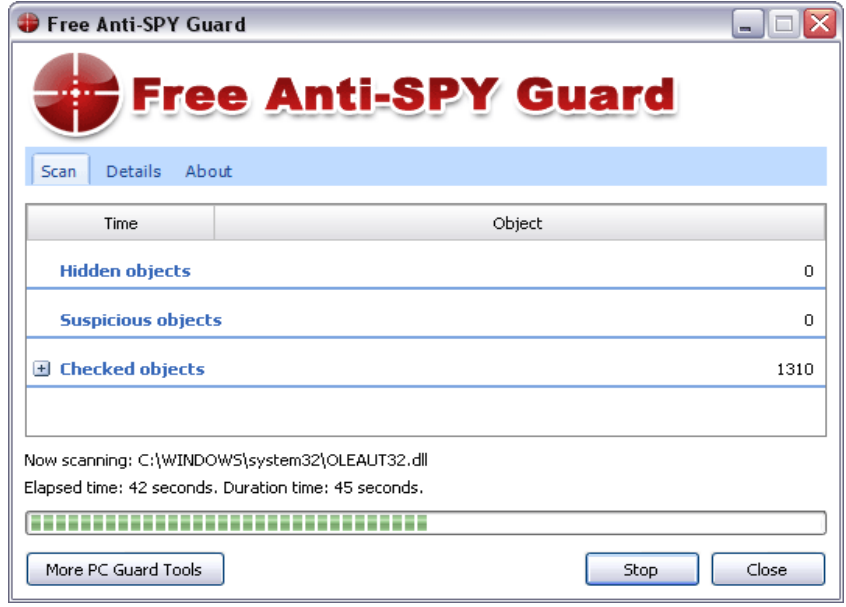
\includegraphics[width=0.8\linewidth]{freeantispy}
\end{frame}

\begin{frame}{Propagation: Trojan Horse}
  \begin{itemize}
  \item  Based on social engineering
  \item  First identified at NSA in 1972 by Daniel 
    Edwards 
  \item  It's a program with two purposes, one obvious 
    and one hidden from the user 
  \item  Today it's often used to install other software or 
    backdoors 
  \item  Trojan horses can be built from existing 
    programs using a special wrapper 
  \item  Or designed from the start to be one.
  \end{itemize}
\end{frame}

\begin{frame}{Propagation: Worms}
  \begin{itemize}
  \item  replicating program that propagates over net (or SW flaw)
    \begin{itemize}
    \item  using email, remote exec, remote login 
    \end{itemize}
  \item  has phases: 
    \begin{itemize}
    \item  dormant, propagation, triggering, execution 
    \item  propagation phase: searches for other systems, connects to 
      it, copies self to it and runs 
    \end{itemize}
  \item  may disguise itself as a system process 
  \item  implemented by Xerox Palo Alto labs in 1980's
  \end{itemize}
\end{frame}

\begin{frame}{Worms - replication}
  \begin{itemize}
  \item  E-mail
    \begin{itemize}
    \item  target client bugs so that the worm is executed whenever an
      infected mail is received
    \end{itemize}
  \item  File-sharing
    \begin{itemize}
    \item  automatic execution of SW when removable devices are connected
    \end{itemize}
  \item  Remote file access
    \begin{itemize}
    \item  by flaw on the target or licit access
    \end{itemize}
  \item  Remote login
    \begin{itemize}
    \item  by flaw on the target or licit access
    \end{itemize}
  \end{itemize}
\end{frame}

\begin{frame}{Morris Worm}
  \begin{itemize}
  \item  one of best known early worms 
  \item  released by Robert Morris in 1988 
  \item  various attacks on UNIX systems 
    \begin{itemize}
    \item  cracking password file to use login/password to 
      logon to other systems 
    \item  exploiting a bug in the finger protocol 
    \item  exploiting a bug in sendmail 
    \end{itemize}
  \item  if succeed have remote shell access 
    \begin{itemize}
    \item  sent bootstrap program to copy worm over
    \end{itemize}
  \end{itemize}
\end{frame}

\begin{frame}{Worm Propagation Model}
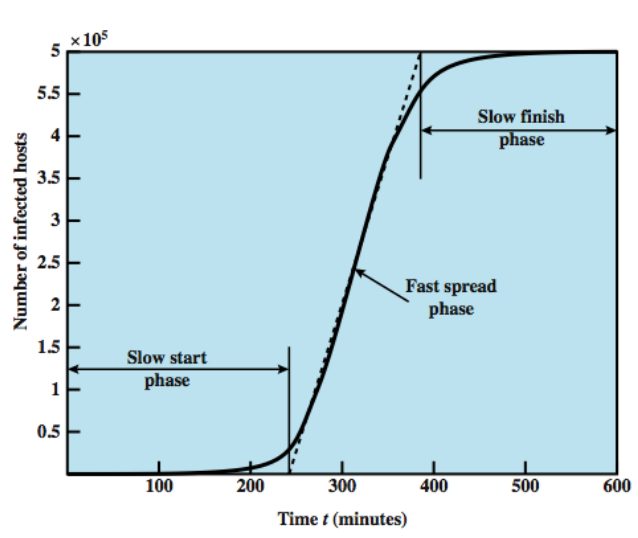
\includegraphics[width=0.8\linewidth]{wormPropagation}
\end{frame}

\begin{frame}{Recent Worm Attacks}
  \begin{itemize}
  \item  Code Red 
    \begin{itemize}
    \item  July 2001 exploiting MS IIS bug 
    \item  probes random IP address, does DDoS attack 
    \item  consumes significant net capacity when active 
    \end{itemize}
  \item  Code Red II variant includes backdoor 
  \item  SQL Slammer 
    \begin{itemize}
    \item  early 2003, attacks MS SQL Server 
    \item  compact and very rapid spread 
    \end{itemize}
  \item  Mydoom 
    \begin{itemize}
    \item  mass-mailing e-mail worm that appeared in 2004 
    \item  installed remote access backdoor in infected systems 
    \end{itemize}
  \item Stuxnet
  \end{itemize}
\end{frame}

\begin{frame}{Worm Technology}
  \begin{itemize}
  \item  multiplatform 
  \item  multi-exploit 
  \item  ultrafast spreading 
  \item  transport vehicles 
  \item  zero-day exploit
  \end{itemize}
\end{frame}

\begin{frame}{Propagation: Viruses }
  \begin{itemize}
  \item  piece of software that infects programs 
    \begin{itemize}
    \item  modifying them to include a copy of the virus 
    \item  so it executes secretly when host program is run 
    \end{itemize}
  \item  specific to operating system and hardware 
    \begin{itemize}
    \item  taking advantage of their details and weaknesses 
    \end{itemize}
  \item  a typical virus goes through phases of: 
    \begin{itemize}
    \item  dormant 
    \item  propagation 
    \item  triggering 
    \item  execution
    \end{itemize}
  \end{itemize}
\end{frame}

\begin{frame}{Virus Structure }
  \begin{itemize}
  \item  components: 
    \begin{itemize}
    \item  infection mechanism - enables replication 
    \item  modification engine - for disguise 
    \item  trigger - event that makes payload activate 
    \item  payload - what it does, malicious or benign 
    \end{itemize}
  \item  when infected program invoked, executes 
    virus code then original program code 
  \item  can block initial infection (difficult)‏ 
  \item  or propagation (with access controls)
  \end{itemize}
\end{frame}

\begin{frame}[fragile]{Naive virus structure}
  \begin{verbatim}
0x00000000 goto main;
0x00000004 666;
main:      infect();
           if trigger() then do-damage();
           goto victim:
infect:    file = get-random-exec();
           if file[0x00000004] = 666 goto infect;
           prepend V to file;
           return;
do-damage: ...
trigger:   ...
victim:    ...
  \end{verbatim}
\end{frame}


\begin{frame}{Virus Classification}
  \begin{itemize}
  \item  by target
    \begin{itemize}
    \item  boot sector 
    \item  file infector 
    \item  macro virus 
    \end{itemize}
  \item by strategy
    \begin{itemize}
    \item  encrypted virus: different keys 
    \item  stealth virus: evade detection, e.g. 
      compression 
    \item  polymorphic virus 
    \item  metamorphic virus
    \end{itemize}
  \end{itemize}
\end{frame}

\begin{frame}[fragile]{Compression virus}
  \begin{verbatim}
0x00000000 goto main;
0x00000004 666;
main:      infect();
           if trigger() then do-damage();
           uncompressVictim();
           goto victim:
infect:    file = get-random-exec();
           if file[0x00000004] = 666 goto infect;
           compress file;
           prepend V to file;
           return;
do-damage: ...
trigger:   ...
victim:    ...
  \end{verbatim}
\end{frame}

\begin{frame}{Compression virus}
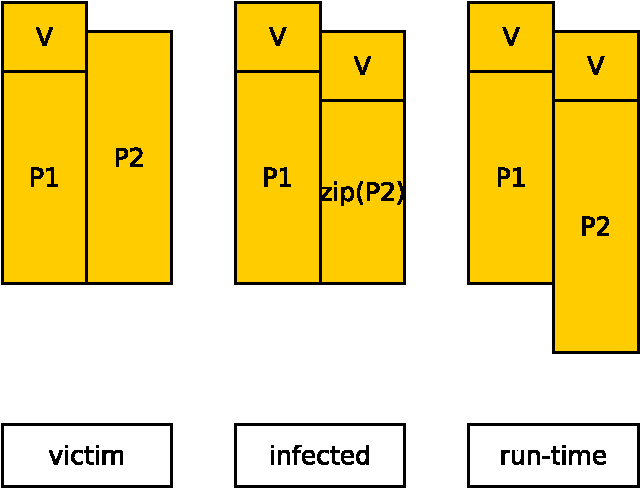
\includegraphics[width=0.8\linewidth]{compressingVirus}
\end{frame}

\begin{frame}{Encrypted virus }
  \begin{itemize}
  \item  Generate key (weak encryption scheme)
  \item  Crypt the virus body
  \item  Copy the bootstrap (decryption engine with key)
    and the encrypted virus body
  \item  When start
  \begin{itemize}
    \item Decrypt the virus body
    \item Execute
  \end{itemize}
  \end{itemize}
\end{frame}

\begin{frame}{Encrypted virus}
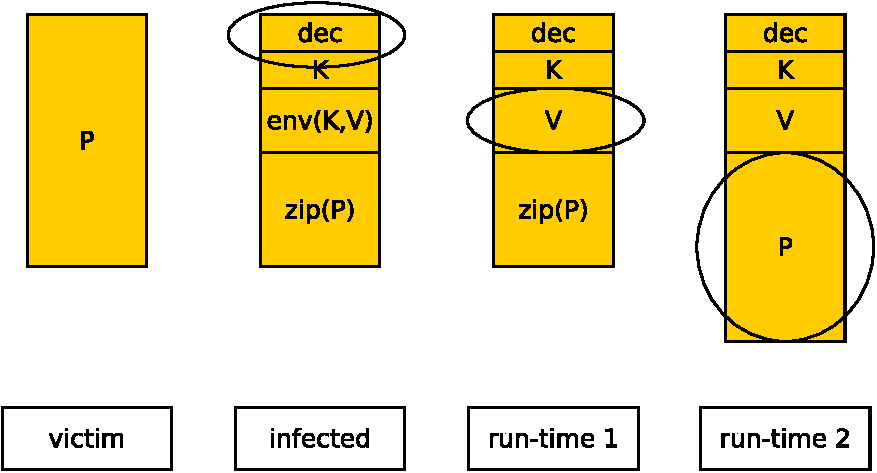
\includegraphics[width=0.8\linewidth]{dec}
\end{frame}


\begin{frame}{Polymorphic Virus }
  \begin{itemize}
  \item A virus can take things one step further: 
    Rebuild the whole virus at every infection to 
    something functionally identical 
  \item There are many ways to do nothing on a 
    computer 
  \item Focus on the decryption engine
  \item Instructions can be reordered in many ways 
  \end{itemize}
\end{frame}

\begin{frame}{Polymorphic virus}
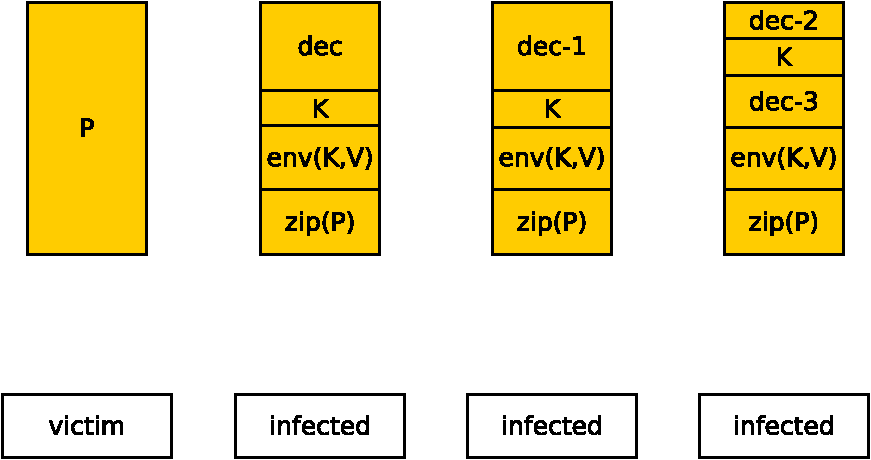
\includegraphics[width=0.8\linewidth]{poly}
\end{frame}

\begin{frame}{Metamorphic Virus}
  \begin{itemize}
  \item  Complete rewrite 
  \item  Can also change behavior
  \item  Techniques useful also for buffer overflow protection
  \end{itemize}
\end{frame}
 
\begin{frame}{Macro Virus }
  \begin{itemize}
  \item  became very common in mid-1990s since 
    \begin{itemize}
    \item  platform independent 
    \item  infects documents 
    \item  is easily spread 
    \end{itemize}
  \item  exploit macro capability of office apps 
    \begin{itemize}
    \item  executable program embedded in office doc 
    \item  often a form of Basic 
    \end{itemize}
  \item  more recent releases include protection 
  \item  recognized by many anti-virus programs 
  \end{itemize}
\end{frame}

\begin{frame}{E-Mail Viruses }
  \begin{itemize}
  \item  more recent development 
  \item  e.g. Melissa 
    \begin{itemize}
    \item  exploits MS Word macro in attached doc 
    \item  if attachment opened, macro activates 
    \item  sends email to all on users address list 
    \item  and does local damage 
    \end{itemize}
  \item  then saw versions triggered reading email 
  \item  hence much faster propagation
  \end{itemize}
\end{frame}


%% Payload


\begin{frame}{Payload: target integrity}
  \begin{itemize}
  \item  Deletion of files, contacts, etc
  \item  Ransomware
    \begin{itemize}
      \item encrypt files
      \item delete files
      \item collect ransom money (e.g. bitcoin)
    \end{itemize}
  \item Physical integrity
    \begin{itemize}
      \item Stuxnet, nuclear centrifuges via compromising  Siemencs
        control software
    \end{itemize}
  \end{itemize}
\end{frame}

\begin{frame}{Payload: Logic Bomb }
  \begin{itemize}
  \item  A small bit of code that triggers on a specific 
    condition 
  \item  Typically with malicious results 
  \item  No vector for spreading 
  \item  Installed directly
  \end{itemize}
\end{frame}

\begin{frame}{Payload: Bots}
  \begin{itemize}
  \item  program taking over other computers 
  \item  to launch hard to trace attacks 
  \item  if coordinated form a botnet 
  \item  characteristics: 
    \begin{itemize}
    \item  remote control facility 
    \end{itemize}
  \item  via IRC/HTTP etc 
    \begin{itemize}
    \item  spreading mechanism 
    \end{itemize}
  \item  multi-layered networks of bots
  \end{itemize} 
\end{frame}

\begin{frame}{Payload: Bots}
  \begin{itemize}
  \item  Uses of bots
  \begin{itemize}
  \item  Distributed Denial of Service
  \item  Spamming
  \item  Manipulating on-line pools
  \item  Use computational resources (e.g. bit coin mining, password
    brute forcing)
  \item Spreading new malware
  \end{itemize}
  \end{itemize}
\end{frame}

\begin{frame}{Payload: information theft}
  \begin{itemize}
  \item  Key loggers
  \item  Spyware
  \item  Phishing
  \item  Espionage
  \end{itemize}
\end{frame}

\begin{frame}{Payload: Backdoor}
  \begin{itemize}
  \item  Software that gives access to a system 
  \item  Bypassing OS restrictions 
  \item  Can be part of a trojan 
  \item  Often installed for legitimate reasons 
  \item  Only to later be abused 
  \item  Typically very very hard to find
  \end{itemize}
\end{frame}

%% \begin{frame}{Legitimate Reasons?}
%%   \begin{itemize}
%%   \item  What would be a legitimate reason to install a 
%% backdoor?  
%%   \end{itemize}
%% \end{frame}

\begin{frame}{Payload: Rootkits}
  \begin{itemize}
  \item  set of programs installed for admin access 
  \item  malicious and stealthy changes to host O/S 
  \item  may hide its existence 
    \begin{itemize}
    \item  subverting report mechanisms on processes, files, registry entries 
      etc 
    \end{itemize}
  \item  may be: 
    \begin{itemize}
    \item  persistent or memory-based 
    \item  user or kernel mode 
    \end{itemize}
  \item  installed by user via trojan or intruder on system 
  \item  range of countermeasures needed
  \item Sony BMG copy protection rootkit and trojan
  \end{itemize}
\end{frame}

\begin{frame}{Rootkits}
  \begin{itemize}
  \item  User mode
  \begin{itemize}
    \item Dynamically patch user processes
    \item Patch dynamically linked libraries
  \end{itemize}
  \item  Kernel mode
  \begin{itemize}
    \item Patch kernel code
    \item Patch kernel system table
    \item Patch kernel interrupt vector
  \end{itemize}
  \item  Hypervisor
  \begin{itemize}
    \item Uses free privileged ring
  \end{itemize}
  \end{itemize}
\end{frame}

\begin{frame}{Rootkit System Table Mods}
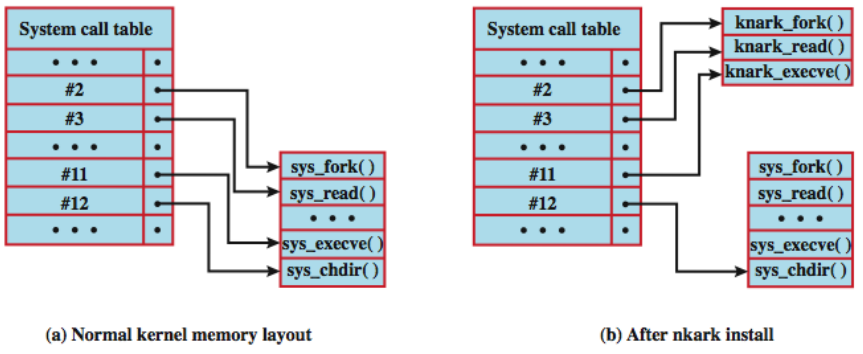
\includegraphics[width=0.8\linewidth]{rootkit}
\end{frame}

\begin{frame}{Reading a file}
  \begin{enumerate}
  \item  User process invokes ``fscanf'' from libc
  \begin{itemize}
    \item \alert<2>{libc is in the process memory (static link)}
    \item \alert<3>{libc is shared among all processes (dynamic link)}
  \end{itemize}
  \item  \alert<2-3>{libc processes the request}
  \item  libc invokes the ``sys\_read'' call
    \begin{enumerate}
      \item \alert<2-3>{libc prepares the syscall parameters}
      \item \alert<2-3>{libc executes the software interrupt}
      \item \alert<7>{CPU switches to privileged mode, PC = vector table + 8}
      \item \alert<4>{jmp to the software interrupt handler}
      \item \alert<6>{infer the invoked syscall address by looking the
        parameters and the system table}
      \item \alert<5>{call ``sys\_read''}
      \item return to the calling user process
    \end{enumerate}
  \item  \alert<2-3>{libc processes the response}
  \end{enumerate}
\end{frame}


%%% countermeasures

\begin{frame}{Countermeasure - prevention: code signing}
  \begin{itemize}
  \item  Used in digital SW distribution (e.g. Debian APT, Android
    play store)
  \item  Used by HW vendor to prevent execution of arbitrary SW (e.g. XBox)
  \item  Used by OSes to install binary drivers (e.g. Windows)
  \item  SW shipped with a digital certificate
    \begin{itemize}
    \item e.g. $cert=Enc(PR_{google}, Hash(SW))$
    \item check $Dec(PU_{google}, cert) = Hash(SW)$
    \end{itemize}
  \item Root of trust
    \begin{itemize}
      \item HW $\rightarrow$ bootloader $\rightarrow$ OS $\rightarrow$
        app $\rightarrow$ plug-in
    \end{itemize}
  \end{itemize}
\end{frame}

\begin{frame}{Countermeasure - prevention/detection}
  \begin{itemize}
  \item  Intrusion Detection/Prevention Systems
  \item  At network level (e.g. to temporarily prevent a worm
    infection due to a know bug)
  \item  At application level (e.g. SMTP servers inspecting mails)
  \end{itemize}
\end{frame}


\begin{frame}{Countermeasures}
  \begin{itemize}
  \item  prevention - ideal solution but difficult 
  \item  realistically need: 
    \begin{itemize}
    \item  detection 
    \item  identification 
    \item  removal 
    \end{itemize}
  \item  if detected but can't identify or remove, must 
    discard and replace infected program
  \end{itemize}
\end{frame}

  %% \item To detect these the AV engine often has to 
  %%   simulate the virus to figure out what it is.
  %% \item Sandboxing techniques


\begin{frame}{Anti-Virus Evolution }
  \begin{itemize}
  \item  virus \& antivirus tech have both evolved 
  \item  early viruses simple code, easily removed 
  \item  as become more complex, so must the 
    countermeasures 
  \item  generations 
    \begin{itemize}
    \item  first - signature scanners 
    \item  second - heuristics 
    \item  third - identify actions 
    \item  fourth - combination packages 
    \end{itemize}
  \end{itemize}
\end{frame}

\begin{frame}{Generic Decryption }
  \begin{itemize}
  \item  runs executable files through GD scanner: 
    \begin{itemize}
    \item  CPU emulator to interpret instructions 
    \item  virus scanner to check known virus signatures 
    \item  emulation control module to manage process 
    \end{itemize}
  \item  lets virus decrypt itself in interpreter 
  \item  periodically scan for virus signatures 
  \item  issue is long to interpret and scan 
    \begin{itemize}
    \item  tradeoff chance of detection vs time delay
    \end{itemize}
  \item virtualization
  \end{itemize}
\end{frame}




%% \begin{frame}{Digital Immune Systems}
%% 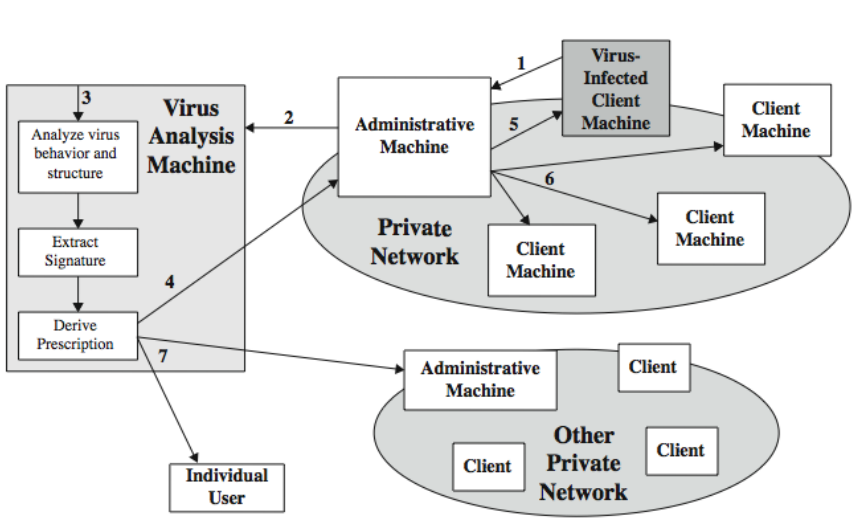
\includegraphics[width=0.8\linewidth]{digitalImmuneSystem}
%% \end{frame}

\begin{frame}{Behavior-Blocking Software}
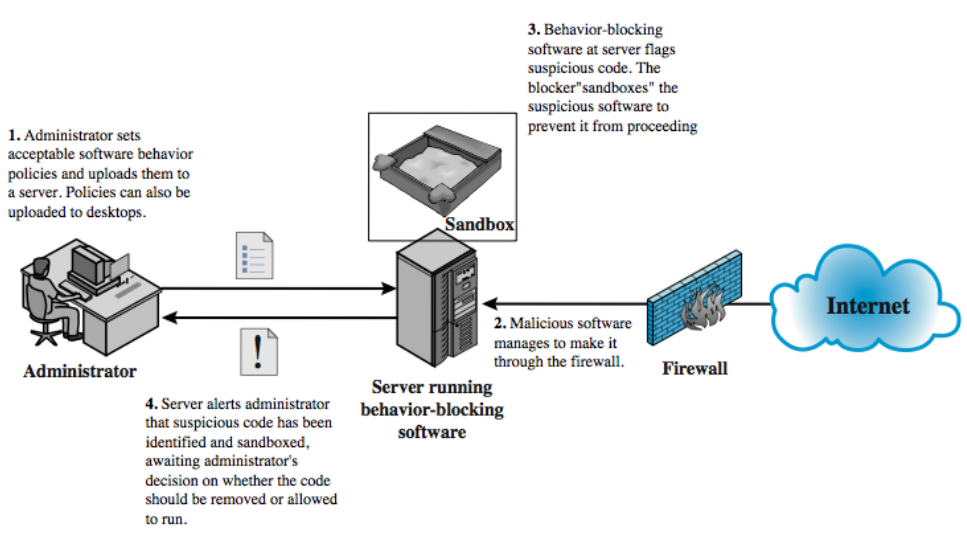
\includegraphics[width=0.8\linewidth]{behaviorBlocking}
\end{frame}

\begin{frame}{Behavior-Blocking Software}
  Monitor
    \begin{itemize}
    \item  Attempts to access files
    \item  Attempts to perform unrecoverable operations (halt, disk format)
    \item  Modification of executable code
    \item  Modification of system settings
    \item  Delivery of documents containing scripts
    \item  Initiation of network communications
    \end{itemize}
    Require complete mediation
\end{frame}

 
\begin{frame}{Worm Countermeasures}
  \begin{itemize}
  \item  overlaps with anti-virus techniques 
  \item  once worm on system A/V can detect 
  \item  worms also cause significant net activity 
  \item  worm defense approaches include: 
    \begin{itemize}
    \item  signature-based worm scan filtering 
    \item  filter-based worm containment 
    \item  payload-classification-based worm containment 
    \item  threshold random walk scan detection 
    \item  rate limiting and rate halting 
    \end{itemize}
  \item Support from perimeter scanning (e.g. network monitor,
    physical monitor of USB sticks)
  \end{itemize}
\end{frame}

\begin{frame}{Proactive Worm Containment}
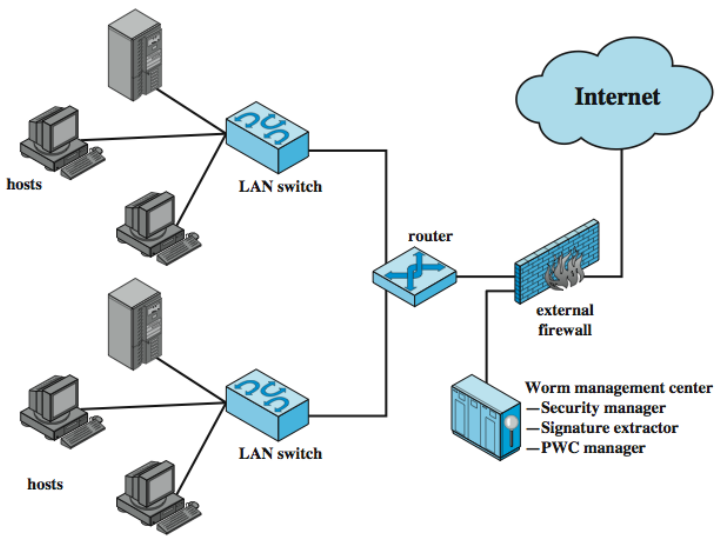
\includegraphics[width=0.8\linewidth]{wormContaiment}
\end{frame}

\begin{frame}{Stuxnet}
  \begin{center}
    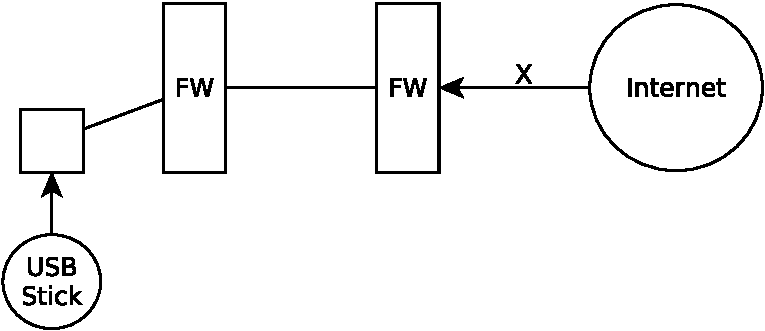
\includegraphics[width=0.7\linewidth]{stuxnet1}
    \begin{itemize}
    \item   LNK/PIF vulnerability: payload execution accomplished when
      an icon is viewed in Windows Explorer
    \item  kernel-mode rootkit: device drivers digitally signed with
      the (stolen) private keys of Realtek
    \end{itemize}
  \end{center}
\end{frame}

\begin{frame}{Stuxnet}
  \begin{center}
    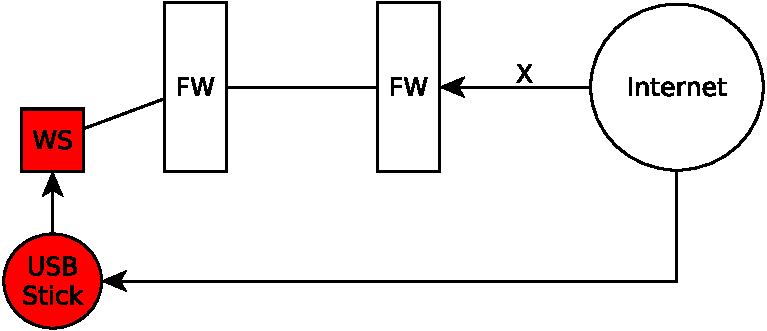
\includegraphics[width=0.7\linewidth]{stuxnet2}
    \begin{itemize}
    \item   LNK/PIF vulnerability: payload execution accomplished when an icon is viewed in Windows Explorer
    \item  kernel-mode rootkit: device drivers digitally signed with
      the (stolen) private keys of Realtek
    \end{itemize}
  \end{center}
\end{frame}

\begin{frame}{Stuxnet}
  \begin{center}
    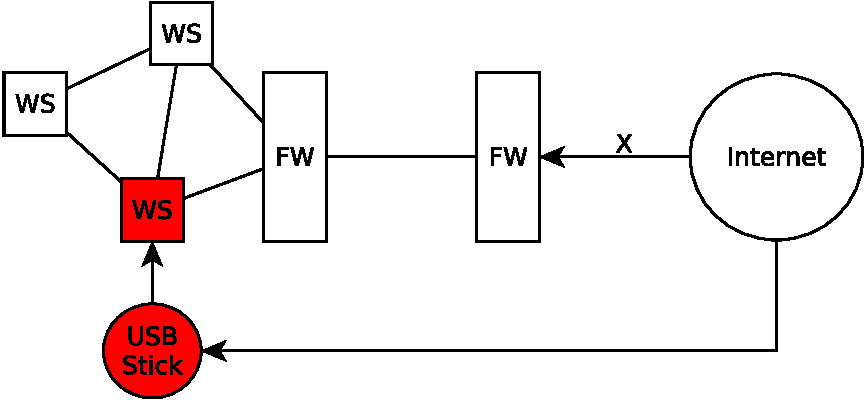
\includegraphics[width=0.7\linewidth]{stuxnet3}
    \begin{itemize}
    \item Remote (LAN) code execution by exploiting Microsoft Printer
      Sharing flaw
    \end{itemize}
  \end{center}
\end{frame}


\begin{frame}{Stuxnet}
  \begin{center}
    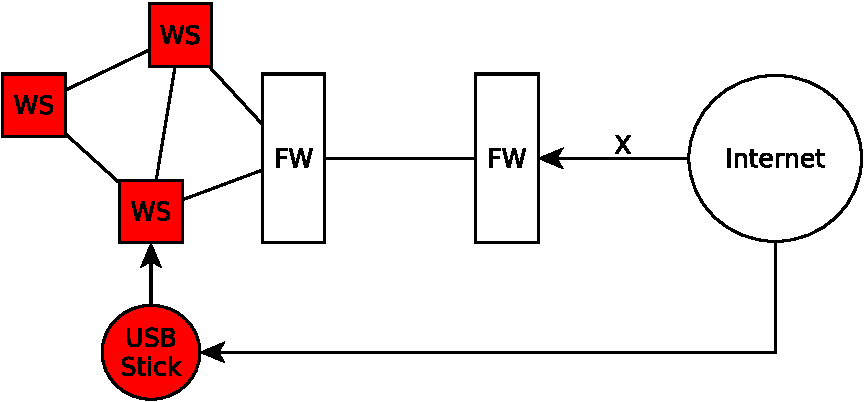
\includegraphics[width=0.7\linewidth]{stuxnet4}
    \begin{itemize}
    \item Remote (LAN) code execution by exploiting Microsoft Printer
      Sharing flaw
    \end{itemize}
  \end{center}
\end{frame}

\begin{frame}{Stuxnet}
  \begin{center}
    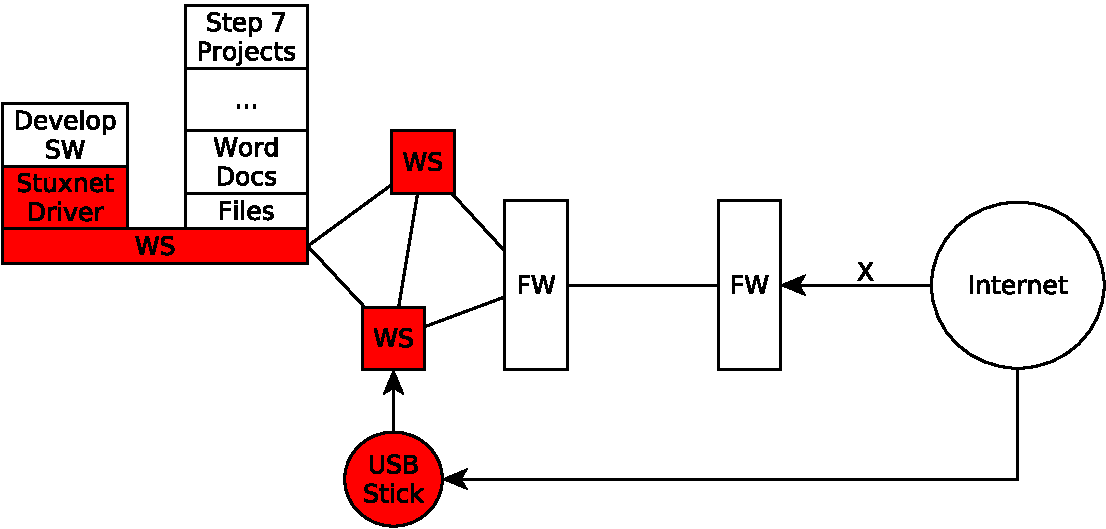
\includegraphics[width=0.7\linewidth]{stuxnet5}
    \begin{itemize}
    \item Infects project files belonging to Siemens' WinCC/PCS 7 SCADA control software
    \end{itemize}
  \end{center}
\end{frame}

\begin{frame}{Stuxnet}
  \begin{center}
    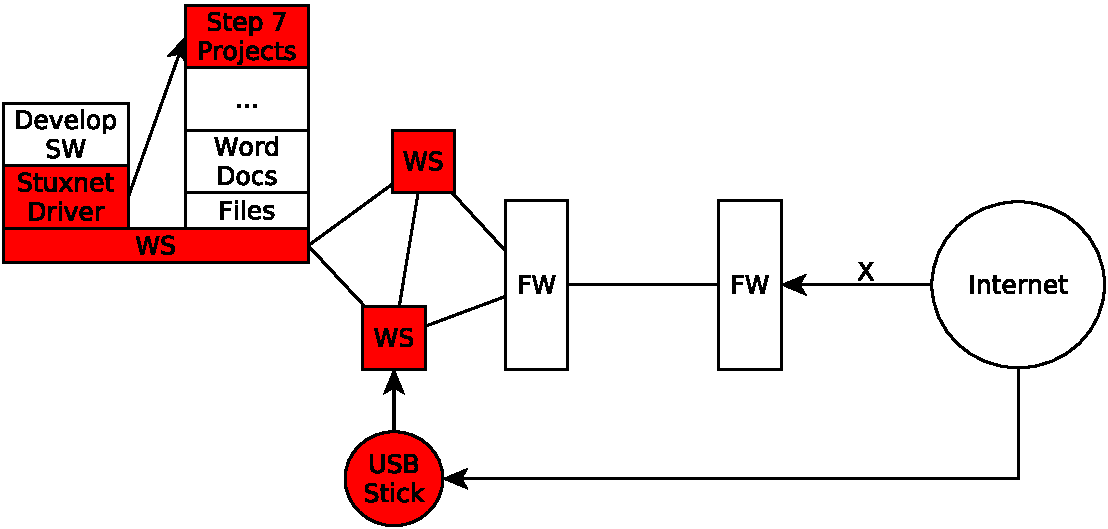
\includegraphics[width=0.7\linewidth]{stuxnet6}
    \begin{itemize}
    \item Infects project files belonging to Siemens' WinCC/PCS 7 SCADA control software
    \end{itemize}
  \end{center}
\end{frame}

\begin{frame}{Stuxnet}
  \begin{center}
    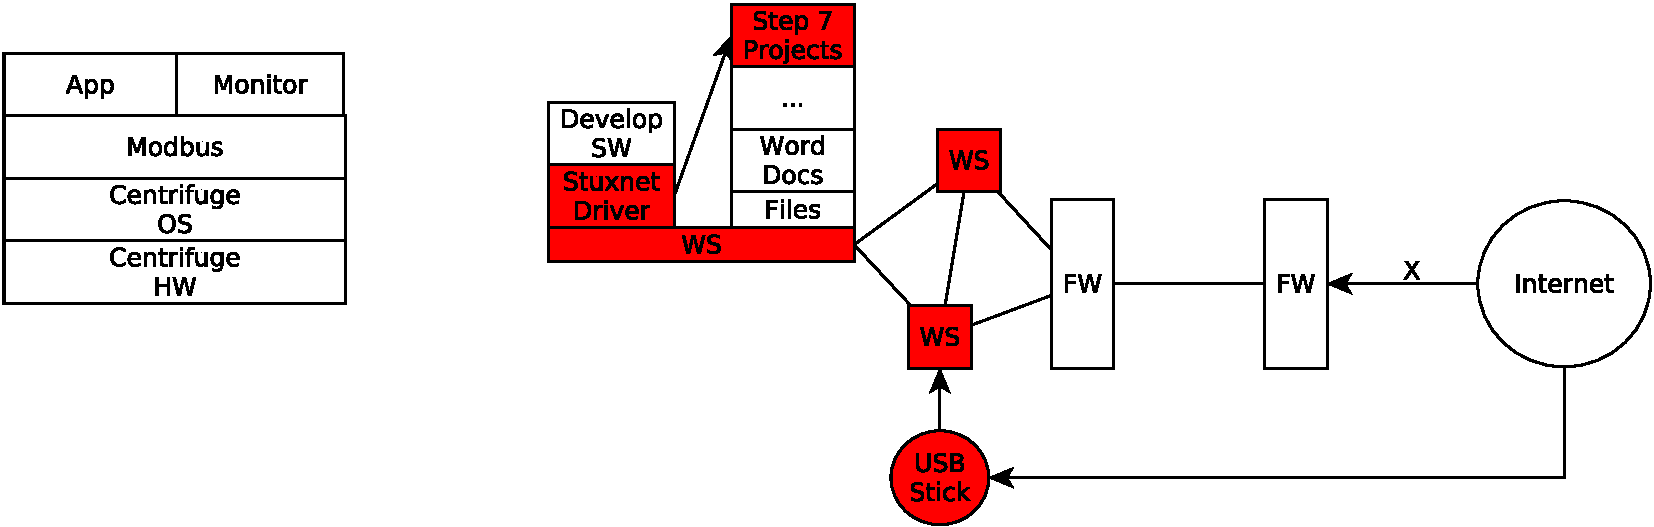
\includegraphics[width=0.7\linewidth]{stuxnet7}
    \begin{itemize}
    \item Infects project files belonging to Siemens' WinCC/PCS 7 SCADA control software
    \end{itemize}
  \end{center}
\end{frame}

\begin{frame}{Stuxnet}
  \begin{center}
    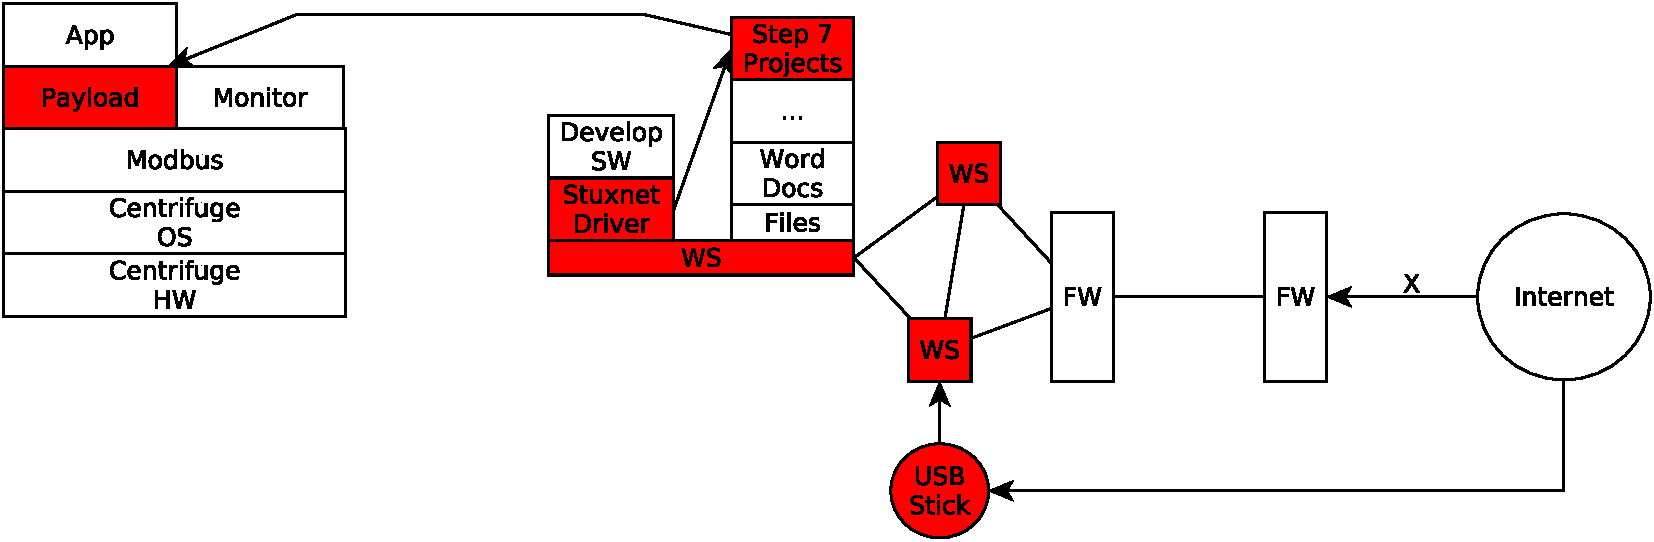
\includegraphics[width=0.7\linewidth]{stuxnet8}
    \begin{itemize}
    \item When certain criteria are met, modifies the motor frequency
    \end{itemize}
  \end{center}
\end{frame}

\begin{frame}{Stuxnet}
  \begin{center}
    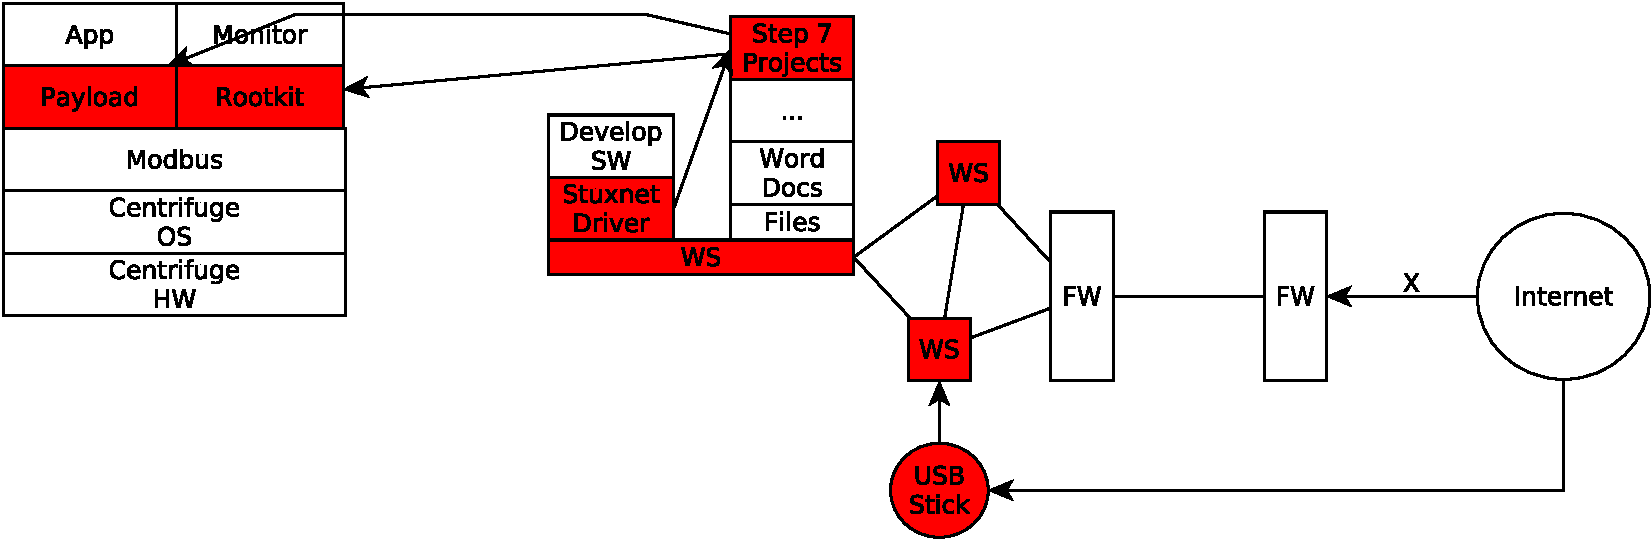
\includegraphics[width=0.7\linewidth]{stuxnet9}
    \begin{itemize}
    \item Hides the changes in rotational speed from monitoring systems.
    \end{itemize}
  \end{center}
\end{frame}

\end{document}




%%% Local Variables: 
%%% mode: latex
%%% TeX-master: t
%%% End: 
